%% 
%% Copyright 2019-2024 Elsevier Ltd
%% 
%% This file is part of the 'CAS Bundle'.
%% --------------------------------------
%% 
%% It may be distributed under the conditions of the LaTeX Project Public
%% License, either version 1.3c of this license or (at your option) any
%% later version.  The latest version of this license is in
%%    http://www.latex-project.org/lppl.txt
%% and version 1.3c or later is part of all distributions of LaTeX
%% version 1999/12/01 or later.
%% 
%% The list of all files belonging to the 'CAS Bundle' is
%% given in the file `manifest.txt'.
%% 
%% Template article for cas-dc documentclass for 
%% double column output.

% Adapted for SGTG stage-2 faithful migration. Local XeLaTeX, no journal-compliance claim.
% !TeX program = xelatex
\documentclass[a4paper,fleqn]{cas-dc}
\usepackage[numbers]{natbib}
\usepackage{cas-xetex-compat}
\usepackage{sgtg-floats}
\usepackage{sgtg-final-layout}
\setlength{\emergencystretch}{3em}
\begin{document}
\let\WriteBookmarks\relax
\def\floatpagepagefraction{1}
\def\textpagefraction{.001}
% Citation numbers are generated from actual manuscript citations (no forced nocite order).
% Stage 3: author identities rechecked against the old author source; see author_reference_review.md.
% DOCX body[0]: title; original line break converted to whitespace.
\shorttitle{SGTG \textbar{} Audio-Visual Generalized Zero-Shot Learning}
\shortauthors{H. Wang et al.}
\title[mode=title]{SGTG: Semantic-Guided Gaussian Temporal Grounding for Audio-Visual Generalized Zero-Shot Learning}
\author[1]{Hu Wang}[orcid=0009-0008-1596-5311]
\ead{gs.wanghu24@gzu.edu.cn}
\author[1,2]{Jing Yang}[orcid=0000-0003-1915-9487]
\fnmark[1]
\cormark[1]
\ead{jyang23@gzu.edu.cn}
\author[1]{Xiaoli Ruan}[orcid=0000-0002-7623-3308]
\ead{xlruan@gzu.edu.cn}
\author[1]{Yuling Chen}[orcid=0000-0002-8674-8356]
\ead{ylchen3@gzu.edu.cn}
\author[3]{Xinru Yi}[orcid=0009-0007-4224-4774]
\ead{cme.xryi23@gzu.edu.cn}
\author[4]{Chengjiang Li}[orcid=0000-0002-1864-2023]
\ead{cjli3@gzu.edu.cn}
\author[1,2]{Minyi Guo}[orcid=0000-0003-0034-2302]
\fnmark[2]
\ead{myguo@gzu.edu.cn}
\affiliation[1]{organization={State Key Laboratory of Public Big Data, Guizhou University},city={Guiyang},postcode={550025},country={China}}
\affiliation[2]{organization={Department of Computer Science and Engineering, Shanghai Jiao Tong University},city={Shanghai},postcode={200240},country={China}}
\affiliation[3]{organization={School of Mechanical Engineering, Guizhou University},city={Guiyang},state={Guizhou},postcode={550025},country={China}}
\affiliation[4]{organization={School of Management, Guizhou University},city={Guiyang},postcode={550025},country={China}}
\cortext[1]{Corresponding author}
% Identities explicitly present in the old author source; current applicability pending confirmation.
\fntext[1]{Member, IEEE.}
\fntext[2]{Fellow, IEEE.}
% No old funding, acknowledgments, CRediT, conflicts, or biographies are copied.
% DOCX body[1]: complete original abstract, only the displayed label is replaced by the CAS heading.
\begin{abstract}
Audio-visual generalized zero-shot learning aims to recognize both seen and unseen classes by jointly exploiting audio, visual, and class-semantic information. Although methods such as AVCA and ClipClap-GZSL have made progress in audio-visual representation learning, discriminative actions or sounds may occur only within short temporal intervals. These cues can be missed during feature sampling or diluted by global aggregation, thereby limiting recognition of unseen classes. Besides, insufficient separation between similar class embeddings, weak audio-visual correspondence, and modality-specific noise further hinder generalization. In this paper, we propose SGTG, a semantic-guided Gaussian temporal grounding framework that uses class semantics as a conditioning signal throughout temporal encoding, modality interaction, and fusion. First, we construct initial class embeddings (class prototypes) from fine-grained visual and auditory descriptions using the CLIP and CLAP text encoders. We then perform class embedding optimization to balance class separability and semantic preservation, providing transferable semantic queries for class-conditioned temporal aggregation. Second, we design a class-conditioned Gaussian temporal aggregation module that conditions audio-visual sequences on class semantics and employs independent Gaussian experts with adaptive routing for each modality. This design continuously localizes and aggregates class-relevant segments along the two temporal axes, reducing the dilution of discriminative evidence by redundant background content. Finally, we decouple intra-modal and inter-modal interactions and introduce a sample- and class-conditioned gate to dynamically combine intra-modal representations, inter-modal representations, and direct temporal evidence. This mechanism suppresses modality interference while retaining complementary information. Experiments on VGGSound-GZSL\textsuperscript{\textit{cls}}, UCF-GZSL\textsuperscript{\textit{cls}}, and ActivityNet-GZSL\textsuperscript{\textit{cls}} show that SGTG outperforms the compared methods in the harmonic mean (HM) of seen- and unseen-class mean class accuracies on all three benchmarks, achieving a better balance between seen-class recognition and unseen-class generalization.
\end{abstract}
% DOCX body[2]: all original keywords.
\begin{keywords}
Zero-shot learning \sep Audio-visual learning \sep Video classification \sep Gaussian temporal aggregation
\end{keywords}

\maketitle
\hypersetup{pdfsubject={Audio-visual generalized zero-shot learning manuscript}}
% !TeX root = ../main.tex

% DOCX body[3]
\section{Introduction}\label{sec:introduction}



% DOCX body[4]
Audio-visual generalized zero-shot learning (AVGZSL) jointly exploits the visual and audio streams of a video and establishes associations between audio-visual representations and textual class semantics. The goal is to recognize unseen classes that are absent from training while retaining the ability to distinguish seen classes. Representative methods, including CJME \cite{parida2020cjme}, AVGZSLNet \cite{mazumder2021avgzslnet}, AVCA \cite{mercea2022avca}, and ClipClap-GZSL \cite{kurzendorfer2024clipclap}, have attracted considerable attention in multimodal video understanding and demonstrated promising potential for unseen-class classification.

% DOCX body[5]
Most existing methods follow an \textquotedblleft{}encode first, match later\textquotedblright{} paradigm. They first extract visual and audio features using pre-trained models, encode these features into class-agnostic global representations with temporal Transformers (Fig.~\ref{fig:comparison}(a)) \cite{mercea2022tcaf} or cross-attention mechanisms (Fig.~\ref{fig:comparison}(b)) \cite{mercea2022avca}, and finally align the resulting representations with class label embeddings in a joint embedding space. However, this paradigm has three limitations. First, class semantics participate only in the final matching stage. Critical actions and sounds often occupy only a small portion of a long video, whereas class-irrelevant backgrounds, silence, and redundant movements dilute the discriminative evidence during uniform pooling. Second, although class label embeddings encode semantic relationships, they are not optimized for the target classification task. Closely situated class embeddings of similar classes consequently produce ambiguous decision boundaries. Third, audio and visual features are often concatenated directly or combined using a fixed fusion scheme. When the modalities are weakly correlated or one is noisy, irrelevant information can interfere across modalities and induce modality bias toward seen classes.



% DOCX body[12]
% DOCX body[12]
\begin{figure*}[pos=t]
\centering
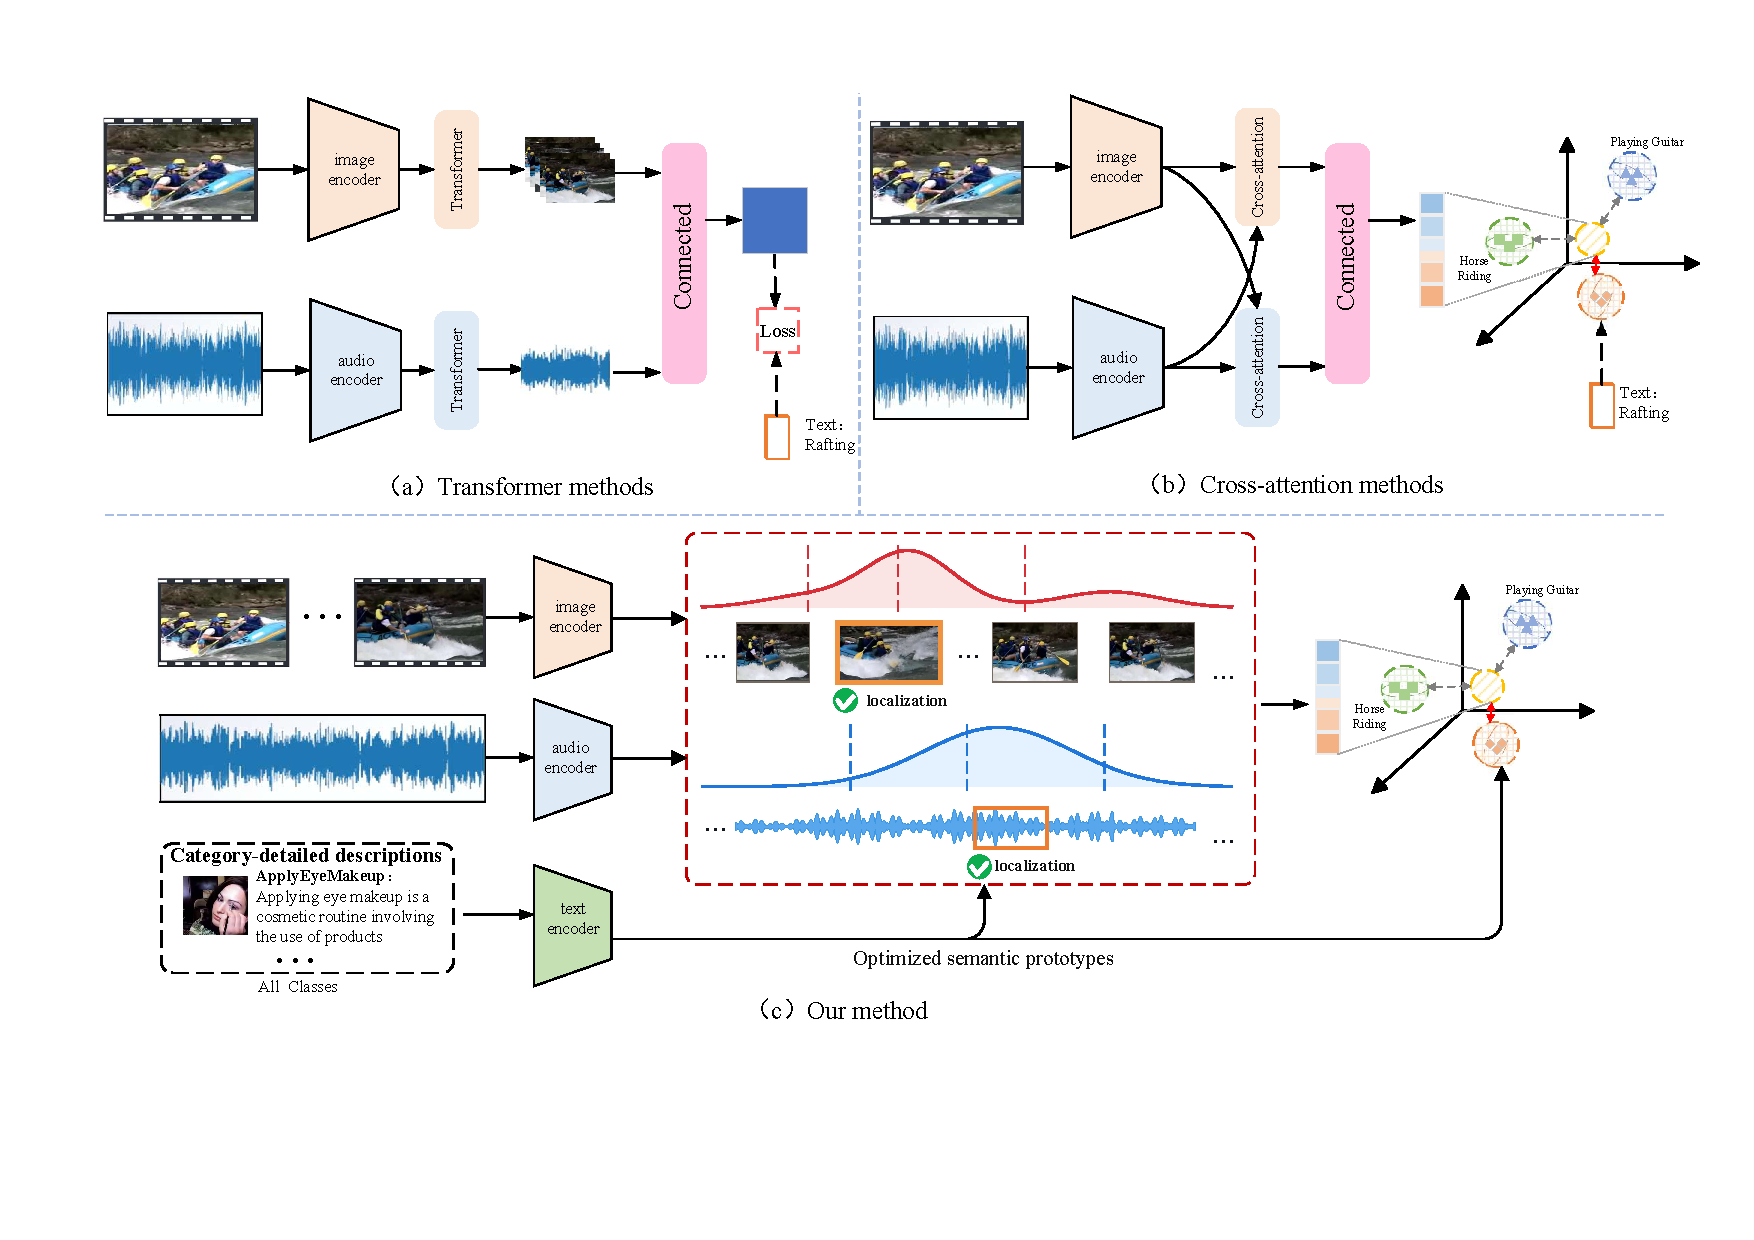
\includegraphics[pagebox=mediabox,width=\textwidth,trim={43bp 99bp 20bp 29bp},clip]{figures/Introduction.pdf}
\caption{Comparison of the proposed framework with existing AVGZSL methods. Transformer-based methods (a) emphasize intra-modal temporal modeling, whereas cross-attention-based methods (b) emphasize inter-modal interaction. Both follow the \textquotedblleft{}encode first, match later\textquotedblright{} paradigm without direct class-semantic guidance for temporal evidence selection. In contrast, our method (c) uses optimized class embeddings to guide independent Gaussian temporal aggregation for visual and audio sequences, adaptively localizes and aggregates class-relevant segments, and aligns the fused audio-visual representation with the class embeddings.}
\label{fig:comparison}
\end{figure*}


% DOCX body[6]
In this paper, we reconsider the role of class semantics in the recognition pipeline. Rather than treating semantics as static class embeddings used only for matching, we use them as active conditioning signals throughout temporal encoding, audio-visual grounding, and modality fusion. To this end, we propose SGTG, a framework for Semantic-Guided Gaussian Temporal Grounding for Audio-Visual Generalized Zero-Shot Learning. At its core, Class-Conditioned Gaussian Temporal Aggregation (CGTA) uses class-semantic queries to generate separate Gaussian distributions with predicted offsets from initial centers for the visual and audio sequences. Together with sample-adaptive routing weights, these distributions continuously localize, weight, and aggregate class-relevant segments. To provide reliable and transferable queries, we introduce Discriminative Semantic Prototype Optimization (DSPO), which improves class separability while preserving semantic structure. We further design Decoupled Modality Interaction and Gated Fusion (DMIF) to organize the aggregated evidence through separate intra-modal and inter-modal relationships. By adjusting fusion weights according to the sample and candidate class, DMIF makes effective use of the selected evidence.

% DOCX body[7]
These designs yield an AVGZSL framework centered on temporal grounding. Our main contributions are summarized as follows:

\begin{enumerate}
\renewcommand{\labelenumi}{(\arabic{enumi})}

% DOCX body[8]
\item We propose class-conditioned Gaussian temporal aggregation, which generates continuous Gaussian distributions conditioned on transferable class semantics and independently localizes and aggregates class-relevant segments along the visual and audio timelines.

% DOCX body[9]
\item We develop DSPO to optimize class embeddings under two competing objectives: class separability and semantic preservation. The learned class embeddings serve as both discriminative classification references and reliable queries for class-conditioned temporal aggregation.

% DOCX body[10]
\item We design decoupled modality interaction and gated fusion. Complementary attention masks separate intra-modal from inter-modal relationships, while candidate-class conditioning enables three-way adaptive weighting of intra-modal representations, inter-modal representations, and direct temporal evidence. This design mitigates interference caused by weak audio-visual correspondence and modality noise.

% DOCX body[11]
\item Experiments on three AVGZSL benchmarks, namely VGGSound-GZSL\textsuperscript{\textit{cls}}, UCF-GZSL\textsuperscript{\textit{cls}}, and ActivityNet-GZSL\textsuperscript{\textit{cls}}, demonstrate that the proposed model achieves state-of-the-art performance compared with existing methods.

\end{enumerate}

% !TeX root = ../main.tex

% DOCX body[14]
\section{Related Work}\label{sec:related-work}

% DOCX body[15]
\subsection{Audio-Visual Generalized Zero-Shot Learning}\label{sec:audio-visual-generalized-zero-shot-learning}

% DOCX body[16]
The central objective of AVGZSL is to transfer audio-visual knowledge from seen to unseen classes through class semantics. To bridge the modality gap between audio-visual observations and text, Parida et al. \cite{parida2020cjme} construct a shared embedding space in CJME, while Mazumder et al. \cite{mazumder2021avgzslnet} introduce label-feature reconstruction in AVGZSLNet. These approaches strengthen cross-modal correspondence through geometric alignment and semantic preservation, respectively. To address the limited information in class names and the restricted expressiveness of feature representations, Chen et al. \cite{chen2023kda} generate fine-grained descriptions using large language models and adjust training margins according to semantic similarity. Kurzend\"{o}rfer et al. \cite{kurzendorfer2024clipclap} combine pre-trained CLIP and CLAP features with two class label embeddings to improve alignment between audio-visual and textual representations. In addition to richer semantic content, class separability also affects recognition. Mo and Morgado \cite{mo2024easy} jointly optimize class separability and semantic preservation in EZ-AVGZL and use the optimized class embeddings to query audio-visual features and compute non-linear similarity scores.

% DOCX body[17]
Nevertheless, prior studies mainly strengthen alignment between audio-visual representations and class embeddings, leaving continuous temporal distributions and their connection to fusion decisions insufficiently explored. Therefore, SGTG uses candidate-class semantics for both temporal grounding and fusion control. The resulting class embeddings preserve semantic structure while remaining discriminative; they act not only as matching references but also as active queries for extracting and combining local evidence.

% DOCX body[18]
\subsection{Audio-Visual Cross-Modal Interaction and Fusion}\label{sec:audio-visual-cross-modal-interaction-and-fusion}

% DOCX body[19]
Audio-visual fusion must balance modality complementarity against the propagation of irrelevant information. To explicitly model cross-modal correspondence, Mercea et al. \cite{mercea2022avca} exchange audio-visual information through cross-modal attention in AVCA. In more general multimodal sequence learning, Tsai et al. \cite{tsai2019mult} use directional cross-attention to capture dependencies between unaligned sequences. Although these methods promote information exchange, interaction alone does not establish the reliability of the exchanged information. To enable selective interaction, Nagrani et al. \cite{nagrani2021bottlenecks} constrain cross-modal information flow through a small number of bottleneck tokens, while Lin et al. \cite{lin2025semiinn} use Intra-modal Masked Attention (IntraMA) and Inter-modal Masked Attention (InterMA), followed by a dynamic gate mechanism, for multimodal sentiment analysis. Further, Ma et al. \cite{ma2026famav} introduce text-conditioned semantic gating in FAMAV to select semantically relevant audio-visual channels.

% DOCX body[20]
However, restricting the scope of interaction or introducing semantic gating does not directly prevent irrelevant information from corrupting class-relevant evidence during relational modeling. To address this issue, we design DMIF to coordinate grounding and fusion. It models intra-modal and inter-modal relationships separately over the evidence sequences while retaining direct temporal evidence that bypasses the masked attention branches. Thus, fusion operates on discriminative evidence supporting the current class rather than on generic modality features.

% DOCX body[21]
\subsection{Temporal Modeling and Grounding}\label{sec:temporal-modeling-and-grounding}

% DOCX body[22]
Temporal modeling requires not only capturing dependencies between segments but also identifying which segments support the current semantic target. To overcome the inability of temporally averaged representations to exploit dynamic structure, Mercea et al. \cite{mercea2022tcaf} model temporal and cross-modal relationships in TCaF. To suppress redundant segments, Li et al. use question-related cues in PSTP-Net \cite{li2023pstp} and TSPM \cite{li2024tspm} to select key segments and focus computation on more discriminative content. To explicitly represent continuous weights over target-relevant segments, Xiao et al. \cite{xiao2024trust} employ Gaussian masks for soft temporal grounding in visually grounded video question answering. Kim et al. \cite{kim2025qatiger} further propose QA-TIGER, which uses question-aware fusion and temporal integration of Gaussian experts to independently weight and aggregate question-relevant audio and visual segments. Compared with discrete selection, these methods express the locality of evidence through parameterized temporal weights and allow multiple segments to jointly support a prediction.

% DOCX body[23]
For AVGZSL, however, temporal modeling must additionally establish transferable semantic associations between local evidence and candidate classes. Therefore, we propose class-conditioned Gaussian temporal aggregation: class descriptions first condition the audio-visual sequences, and discriminative class embeddings then guide continuous Gaussian weighting independently for the visual and audio streams. This design adaptively aggregates local evidence supporting the current class.

% !TeX root = ../main.tex

% DOCX body[24]
\section{Method}\label{sec:method}

% DOCX body[25]
\subsection{Problem Definition}\label{sec:problem-definition}

% DOCX body[26]
In zero-shot learning, classes are divided into two disjoint sets: seen classes and unseen classes. The model is trained only on samples from seen classes, while unseen classes appear only at test time. As a result, it cannot directly learn the data distributions of unseen classes and must instead use class-level semantic information to transfer audio-visual knowledge learned from seen classes. In the more demanding generalized zero-shot setting, test samples come from the union of seen and unseen classes. The model must generalize to unseen classes, retain discrimination among seen classes, and overcome prediction bias toward seen classes. This setting is therefore considered more representative of practical applications. AVGZSL addresses this problem by jointly using the visual and audio content of videos. Although actions and sound events can corroborate one another, their associations with class semantics vary across samples, making seen-to-unseen transfer more challenging. Formally, let ${\mathcal{C}}_{s}$ and ${\mathcal{C}}_{u}$ denote the sets of seen and unseen classes, respectively, with ${\mathcal{C}}_{s}\cap {\mathcal{C}}_{u}=\emptyset .$ The training set contains audio-visual samples from seen classes and is denoted by $\mathcal{S}=\{({x}_{n}^{v},{x}_{n}^{a},{y}_{n}){\}}_{n=1}^{N},$ where ${x}_{n}^{v}$ and ${x}_{n}^{a}$ are the visual and audio streams of training video $n,$ ${y}_{n}\in {\mathcal{C}}_{s}$ is its ground-truth label, and $N$ is the number of training samples. The objective is to learn a decision function $h:({x}^{v},{x}^{a})\mapsto {\mathcal{C}}_{s}\cup {\mathcal{C}}_{u}$ that correctly classifies test samples from the union of seen and unseen classes.

% DOCX body[27]
\subsection{Overall Architecture}\label{sec:overall-architecture}

% DOCX body[28]
Most existing AVGZSL methods use class label embeddings for classification in the final matching stage, separating video encoding from class semantics. In contrast, our framework uses discriminatively optimized class embeddings as conditioning signals throughout encoding to guide temporal grounding, interaction, and fusion for both modalities, as illustrated in Fig.~\ref{fig:architecture}. The framework comprises three components: DSPO, CGTA, and DMIF. First, DSPO expands class names into fine-grained descriptions, constructs initial class embeddings, and improves class separability while preserving semantic structure. This component addresses insufficient discrimination in pre-trained text embeddings and ambiguous boundaries between similar classes, providing reliable semantic references for subsequent temporal aggregation and alignment. Second, CGTA introduces the optimized class semantics into visual and audio sequence encoding and uses continuous Gaussian distributions to localize and aggregate class-relevant segments, preventing irrelevant segments from diluting key evidence. Finally, DMIF organizes the selected audio-visual evidence through separate intra-modal and inter-modal relationships and adaptively adjusts their fusion weights to mitigate the interference and modality bias associated with direct concatenation.

% DOCX body[29]
% DOCX body[29]
\begin{figure*}[pos=t]
\centering
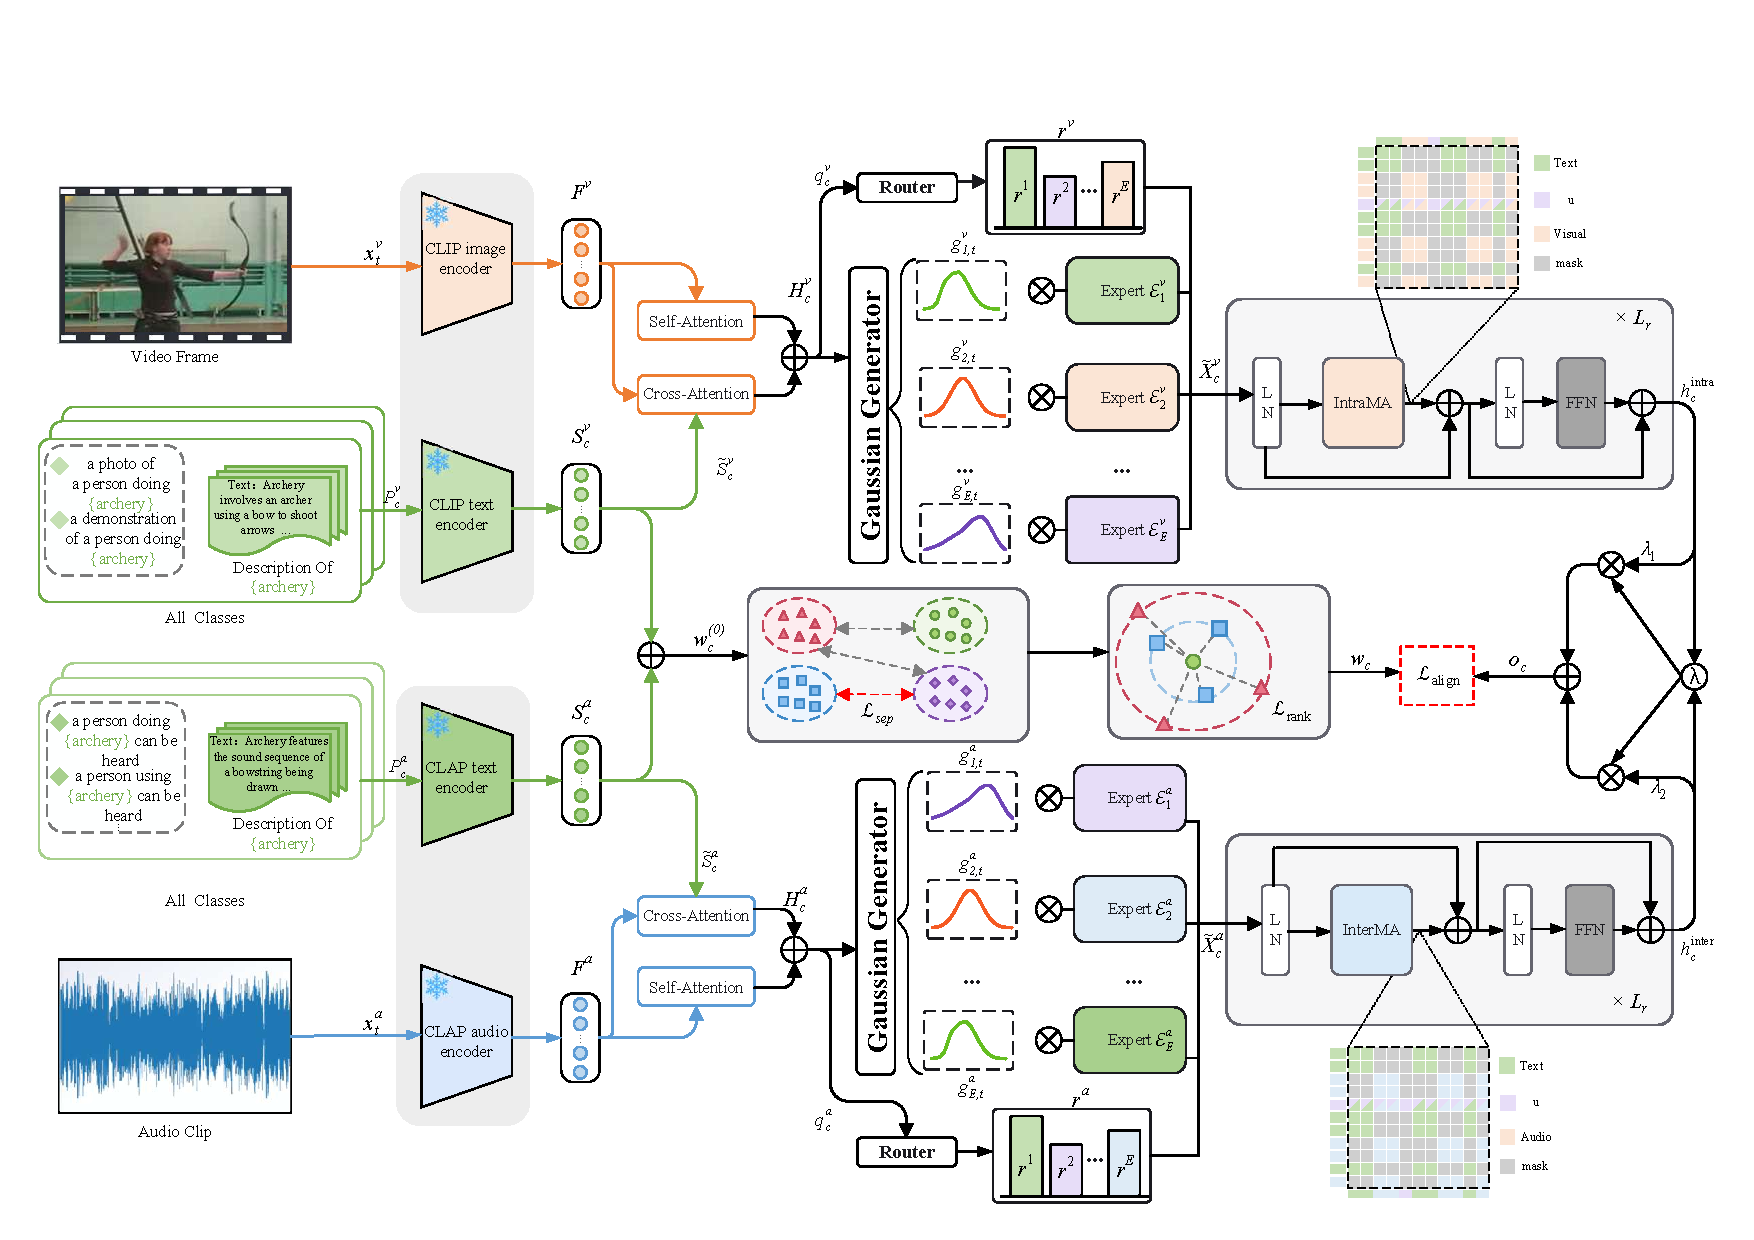
\includegraphics[pagebox=mediabox,width=\textwidth,trim={12bp 11bp 13bp 51bp},clip]{figures/SGTG.pdf}
\caption{Overall architecture of SGTG. An input video is divided into temporally aligned consecutive segments, from which frozen CLIP image and CLAP audio encoders extract visual and audio sequences. In parallel, frozen text encoders transform the candidate class\textquoteright{}s visual and auditory descriptions into description embeddings, and DSPO produces optimized class embeddings that are subsequently fixed. CGTA conditions each modality sequence on its description embeddings and uses the class embedding to query independent visual and audio Gaussian experts with adaptive routing. Continuous weighting and aggregation produce enhanced sequences and direct audio-visual evidence. DMIF then models temporal relationships through intra-modal and inter-modal encoder branches and applies a three-way dynamic Softmax gate conditioned on the direct evidence and candidate class. Finally, a projection network maps the fused representation to a class-conditioned embedding.}
\label{fig:architecture}
\end{figure*}


% DOCX body[31]
\subsection{Discriminative Semantic Prototype Optimization}\label{sec:discriminative-semantic-prototype-optimization}

% DOCX body[32]
Class label embeddings bridge seen and unseen classes in AVGZSL. Embeddings from pre-trained models such as CLIP and CLAP preserve useful semantic relationships. For example, \textquotedblleft{}playing guitar\textquotedblright{} is closer to \textquotedblleft{}playing violin\textquotedblright{} than to \textquotedblleft{}dog barking\textquotedblright{} in semantic space, and such relationships underpin zero-shot transfer. However, these embeddings are not optimized for the target classification task. Class embeddings of semantically similar classes can be too close to distinguish similar actions or sounds. Conversely, maximizing class separability alone tends to push all class embeddings toward an equidistant configuration, erasing the distinction between semantically related and unrelated classes and disrupting the semantic relationships required for transfer. To resolve this conflict, we develop Discriminative Semantic Prototype Optimization (DSPO) based on class embedding optimization \cite{mo2024easy}. Starting from the original text embeddings, DSPO learns class embeddings with improved separability while retaining their semantic relationships. Specifically, it first constructs text embeddings of class descriptions and then jointly optimizes the class embeddings under two competing objectives: class separability and semantic preservation.

% DOCX body[33]
For class $c,$ let ${\mathcal{P}}_{c}^{v}$ and ${\mathcal{P}}_{c}^{a}$ denote its sets of visual and auditory descriptions, respectively, each containing $P$ descriptions. We pass the two sets through the pre-trained CLIP and CLAP text encoders and stack their outputs row-wise to obtain two matrices of description embeddings, with one encoded description per row:

% DOCX body[34]
% DOCX body[34]; M015
\begin{equation}
\label{eq:visual-description-encoding}
{S}_{c}^{v}={\Phi }_{\mathrm{T}}^{v}\left( {\mathcal{P}}_{c}^{v}\right) \in {\mathbb{R}}^{P\times {d}_{t}^{v}}
\end{equation}


% DOCX body[35]
% DOCX body[35]; M016
\begin{equation}
\label{eq:audio-description-encoding}
{S}_{c}^{a}={\Phi }_{\mathrm{T}}^{a}\left( {\mathcal{P}}_{c}^{a}\right) \in {\mathbb{R}}^{P\times {d}_{t}^{a}}
\end{equation}

% DOCX body[36]
\noindent\unskip where ${\Phi }_{\mathrm{T}}^{v}(\cdot )$ and ${\Phi }_{\mathrm{T}}^{a}(\cdot )$ denote the frozen CLIP and CLAP text encoders, respectively, and ${d}_{t}^{v}$ and ${d}_{t}^{a}$ are their text-embedding dimensions. At the class level, we apply ${\ell }_{2}$ normalization to each row of ${S}_{c}^{v}$ and ${S}_{c}^{a}$ and average the normalized rows to obtain the modality-specific class label embeddings ${\overline{s}}_{c}^{v}\in {\mathbb{R}}^{{d}_{t}^{v}}$ and ${\overline{s}}_{c}^{a}\in {\mathbb{R}}^{{d}_{t}^{a}}.$ Concatenating and normalizing these embeddings gives the initial class embedding:

% DOCX body[37]
% DOCX body[37]; M026
\begin{equation}
\label{eq:initial-class-embedding}
{w}_{c}^{(0)}=\frac{\left[ {\overline{s}}_{c}^{v}\Vert {\overline{s}}_{c}^{a}\right] }{{\left\Vert \left[ {\overline{s}}_{c}^{v}\Vert {\overline{s}}_{c}^{a}\right] \right\Vert }_{2}}\in {\mathbb{R}}^{{d}_{s}}
\end{equation}

% DOCX body[38]
\noindent\unskip where $[\cdot \Vert \cdot ]$ denotes vector concatenation, and ${d}_{s}={d}_{t}^{v}+{d}_{t}^{a}$ is the dimensionality of the class embedding space. Row-wise normalization preserves the directional meaning of the averaged vectors, while global normalization places all class embeddings on the unit sphere, allowing class relationships to be characterized by Euclidean distance.

% DOCX body[39]
Starting from these initial class embeddings, we optimize a new set of class embeddings $\{{w}_{c}{\}}_{c\in \mathcal{C}},$ where $\mathcal{C}={\mathcal{C}}_{s}\cup {\mathcal{C}}_{u},$ subject to ${\left\Vert {w}_{c}\right\Vert }_{2}=1.$ To enhance class separability, we maximize the distance from each class embedding to its nearest neighbor by minimizing the following class-separation loss:

% DOCX body[40]
% DOCX body[40]; M032
\begin{equation}
\label{eq:separation-loss}
{\mathcal{L}}_{sep}=-\sum _{c\in \mathcal{C}}\underset{{c}^{\prime }\in \mathcal{C},{c}^{\prime }\ne c}{\mathrm{min}}{\left\Vert {w}_{c}-{w}_{{c}^{\prime }}\right\Vert }_{2}
\end{equation}

% DOCX body[41]
\noindent\unskip where the inner $\mathrm{min}$ selects the closest other class embedding to class $c,$ and the outer summation accumulates the loss over all classes. Because the loss acts only on each class\textquoteright{}s nearest neighbor, it prioritizes separation of the most easily confused class pairs. We further introduce a margin ranking loss for semantic preservation that maintains the relative order of distances between the initial class embeddings. For distinct classes $c,i\in\mathcal{C}$, let $d_{ci}^{(0)}=\lVert w_c^{(0)}-w_i^{(0)}\rVert_2$ and $d_{ci}=\lVert w_c-w_i\rVert_2$ denote the initial and optimized distances, respectively. For pairwise distinct $c,i,j\in\mathcal{C}$, define $\eta_{cij}=\operatorname{sign}(d_{ci}^{(0)}-d_{cj}^{(0)})$, and let $\mathcal{T}$ contain all such ordered triplets. The margin ranking loss is then

% DOCX body[42]
% DOCX body[42]; M035. Equivalent notation; distances/sign defined in body[41].
\begingroup\postdisplaypenalty=10000
\begin{equation}
\label{eq:ranking-loss}
\mathcal{L}_{rank}=\sum_{(c,i,j)\in\mathcal{T}}\max\bigl\{0,\Delta-\eta_{cij}(d_{ci}-d_{cj})\bigr\}.
\end{equation}
\endgroup

% DOCX body[43]
\noindent\unskip where $\Delta >0$ is the margin coefficient, and $sign(\cdot )$ is the sign function. The triple summation in \eqref{eq:ranking-loss} scales cubically with the number of classes. For a large class set, it can be approximated by randomly sampling a fixed number of triplets at each update. We jointly optimize the two objectives using a trade-off coefficient:

% DOCX body[44]
% DOCX body[44]; M038
\begin{equation}
\label{eq:prototype-objective}
\mathcal{L}=\underset{\{{w}_{c}{\}}_{c\in \mathcal{C}},{\left\Vert {w}_{c}\right\Vert }_{2}=1}{\mathrm{min}}(1-\alpha ){\mathcal{L}}_{rank}+\alpha {\mathcal{L}}_{sep}
\end{equation}

% DOCX body[45]
\noindent\unskip where $\alpha \in (0,1)$ balances class separability against semantic preservation. We initialize the class embeddings with ${w}_{c}={w}_{c}^{(0)},$ solve \eqref{eq:prototype-objective} by gradient descent, and renormalize each class embedding onto the unit sphere after every update. Once optimization converges, all class embeddings $\{{w}_{c}\}$ are fixed. The optimized class embeddings serve not only as alignment targets for classification in Section~\ref{sec:joint-embedding-training-and-inference} but also as conditional queries in the next module, guiding the model to actively localize evidence relevant to each candidate class in long audio-visual sequences.

% DOCX body[46]
\subsection{Class-Conditioned Gaussian Temporal Aggregation}\label{sec:class-conditioned-gaussian-temporal-aggregation}

% DOCX body[47]
Not every segment of a long video is relevant to its class. In a \textquotedblleft{}wood thrush calling\textquotedblright{} video, for example, the critical bird call may occupy only a small portion of the audio, with environmental noise dominating the remaining duration. Likewise, the decisive action in \textquotedblleft{}basketball dunk\textquotedblright{} occurs only within a short frame interval. Under the conventional class-agnostic global encoding paradigm, uniform pooling dilutes such local evidence with redundant segments. For an unseen class without training samples, class semantics are particularly important for actively searching potentially relevant temporal regions. To address this problem, we propose Class-Conditioned Gaussian Temporal Aggregation (CGTA), which uses optimized class embeddings as encoding conditions rather than only as matching references. It first injects description embeddings into the visual and audio sequences to condition their representations on the candidate class. It then generates multiple continuous Gaussian distributions to independently localize and aggregate class-relevant segments along the two modality timelines. CGTA adapts question-aware fusion and temporal integration of Gaussian experts \cite{kim2025qatiger} by replacing question features with description embeddings and optimized class embeddings.

% DOCX body[48]
\textbf{Class-semantic-aware early fusion. }We divide each input video into $T$ non-overlapping consecutive temporal segments. Segment $t$ contains a representative image ${x}_{t}^{v}$ and its corresponding audio waveform ${x}_{t}^{a}.$ Frozen pre-trained encoders extract the segment-level visual and audio features:

% DOCX body[49]
% DOCX body[49]; M046
\begin{equation}
\label{eq:visual-feature}
{F}_{t}^{v}={\Phi }_{\mathrm{V}}\left( {x}_{t}^{v}\right) \in {\mathbb{R}}^{{d}_{v}}
\end{equation}


% DOCX body[50]
% DOCX body[50]; M047
\begin{equation}
\label{eq:audio-feature}
{F}_{t}^{a}={\Phi }_{\mathrm{A}}\left( {x}_{t}^{a}\right) \in {\mathbb{R}}^{{d}_{a}}
\end{equation}

% DOCX body[51]
\noindent\unskip where ${\Phi }_{\mathrm{V}}(\cdot )$ and ${\Phi }_{\mathrm{A}}(\cdot )$ denote the CLIP image and CLAP audio encoders, respectively, while ${d}_{v}$ and ${d}_{a}$ are the corresponding feature dimensions. After stacking the segment features in temporal order to form ${F}^{v}\in {\mathbb{R}}^{T\times {d}_{v}}$ and ${F}^{a}\in {\mathbb{R}}^{T\times {d}_{a}},$ we map them into a shared $d$-dimensional space through two learnable linear projections and add temporal positional encodings:

% DOCX body[52]
% DOCX body[52]; M055
\begin{equation}
\label{eq:feature-projection}
V={F}^{v}{W}_{v}+PE,\quad \quad A={F}^{a}{W}_{a}+PE
\end{equation}

% DOCX body[53]
\noindent\unskip where ${W}_{v}\in {\mathbb{R}}^{{d}_{v}\times d}$ and ${W}_{a}\in {\mathbb{R}}^{{d}_{a}\times d}$ are projection matrices, and $PE\in {\mathbb{R}}^{T\times d}$ is a learnable temporal positional encoding. The two sequences share the same positional encodings to preserve segment order and maintain temporal alignment across modalities. For consistent notation, we define standard scaled dot-product attention as

% DOCX body[54]
% DOCX body[54]; M059
\begin{equation}
\label{eq:attention}
Attn(X,Y)=Softmax\left( \frac{X{W}_{Q}{\left( Y{W}_{K}\right) }^{\top }}{\sqrt{{d}_{k}}}\right) Y{W}_{V}
\end{equation}

% DOCX body[55]
\noindent\unskip where $X$ supplies the queries and $Y$ supplies both the keys and values, with ${W}_{Q},{W}_{K}\in {\mathbb{R}}^{d\times {d}_{k}}$ and ${W}_{V}\in {\mathbb{R}}^{d\times d}.$ The $\mathrm{Softmax}$ operation normalizes along the key dimension. We denote self-attention by $SA(X)=Attn(X,X)$ and cross-attention by $CA(X,Y)=Attn(X,Y).$

% DOCX body[56]
We then inject the description embeddings from Section~\ref{sec:discriminative-semantic-prototype-optimization} into the two modality sequences as keys and values. For candidate class $c,$ learnable projections first map the description embeddings to the shared dimensionality: ${\widetilde{S}}_{c}^{v}={S}_{c}^{v}{W}_{s}^{v}\in {\mathbb{R}}^{P\times d}$ and ${\widetilde{S}}_{c}^{a}={S}_{c}^{a}{W}_{s}^{a}\in {\mathbb{R}}^{P\times d},$ where ${W}_{s}^{v}\in {\mathbb{R}}^{{d}_{t}^{v}\times d}$ and ${W}_{s}^{a}\in {\mathbb{R}}^{{d}_{t}^{a}\times d}.$ The class-conditioned sequence encodings are defined as

% DOCX body[57]
% DOCX body[57]; M072
\begin{equation}
\label{eq:conditioned-visual}
{H}_{c}^{v}=V+SA(V)+CA\left( V,{\widetilde{S}}_{c}^{v}\right) 
\end{equation}


% DOCX body[58]
% DOCX body[58]; M073
\begin{equation}
\label{eq:conditioned-audio}
{H}_{c}^{a}=A+SA(A)+CA\left( A,{\widetilde{S}}_{c}^{a}\right) 
\end{equation}

% DOCX body[59]
\noindent\unskip where ${H}_{c}^{v},{H}_{c}^{a}\in {\mathbb{R}}^{T\times d}$ denote the visual and audio sequences conditioned on class $c,$ respectively.

% DOCX body[60]
\textbf{Temporal integration of Gaussian experts. }Given the class-conditioned sequences, we further localize and aggregate class-relevant evidence along the temporal axis. We use Gaussian distributions as soft masks in a Mixture of Experts (MoE) framework, with independent weighted aggregation for audio and visual features. First, the optimized class embedding queries each conditioned sequence to obtain an aggregated representation for each modality conditioned on the candidate class:

% DOCX body[61]
% DOCX body[61]; M076
\begin{equation}
\label{eq:class-queries}
{q}_{c}^{v}=CA\left( \psi ({w}_{c}),{H}_{c}^{v}\right) ,\quad \quad {q}_{c}^{a}=CA\left( \psi ({w}_{c}),{H}_{c}^{a}\right) 
\end{equation}

% DOCX body[62]
\noindent\unskip where $\psi ({w}_{c})={W}_{\psi }{w}_{c}+{b}_{\psi }\in {\mathbb{R}}^{d}$ is a learnable transformation from the ${d}_{s}$-dimensional class embedding space to the shared feature space. Since $\psi ({w}_{c})$ acts as a single-row attention query, the aggregated representations satisfy ${q}_{c}^{v},{q}_{c}^{a}\in {\mathbb{R}}^{d}.$ We then generate distribution parameters for $E$ Gaussian experts in each modality. Using $m\in \{v,a\}$ to index the modality, we define

% DOCX body[63]
% DOCX body[63]; M083
\begin{equation}
\label{eq:gaussian-parameters}
\left[ {\delta }^{m};{\varepsilon }^{m}\right] ={q}_{c}^{m}{W}_{g}^{m}
\end{equation}


% DOCX body[64]
% DOCX body[64]; M084
\begin{equation}
\label{eq:gaussian-centers-widths}
{\mu }_{k}^{m}=\frac{2k-1}{2E}+\frac{1}{2E}\mathrm{tanh}\left( {\delta }_{k}^{m}\right) ,\quad \quad {\sigma }_{k}^{m}=Softplus\left( {\varepsilon }_{k}^{m}\right) 
\end{equation}

% DOCX body[65]
\noindent\unskip where ${W}_{g}^{m}\in {\mathbb{R}}^{d\times 2E}$ is the parameter-generation matrix. Equation \eqref{eq:gaussian-parameters} divides the $2E$-dimensional output into two equal parts: center offsets ${\delta }^{m}\in {\mathbb{R}}^{E}$ and width parameters ${\varepsilon }^{m}\in {\mathbb{R}}^{E},$ where $k=1,\ldots ,E$ indexes the experts, while ${\mu }_{k}^{m}$ and ${\sigma }_{k}^{m}$ are the Gaussian center and standard deviation of expert $k$ on the normalized temporal axis $[0,1].$ The Gaussian soft mask of expert $k$ at time step $t$ and its temporally normalized form are given by

% DOCX body[66]
% DOCX body[66]; M096
\begin{equation}
\label{eq:gaussian-mask}
{g}_{k,t}^{m}=exp\left( -\frac{{\left( t/T-{\mu }_{k}^{m}\right) }^{2}}{2{\left( {\sigma }_{k}^{m}\right) }^{2}}\right) 
\end{equation}


% DOCX body[67]
% DOCX body[67]; M097
\begin{equation}
\label{eq:normalized-mask}
{\widehat{g}}_{k,t}^{m}=\frac{{g}_{k,t}^{m}}{\sum _{{t}^{\prime }=1}^{T}{g}_{k,{t}^{\prime }}^{m}}
\end{equation}

% DOCX body[68]
\noindent\unskip where the mask ${g}_{k,t}^{m}\in \left( 0,1\right] $ peaks at the expert center and decays continuously with temporal distance, while ${\widehat{g}}_{k,t}^{m}$ is normalized along time and sums to $1.$ To determine the contribution of each expert for the current sample and candidate class, a router generates routing values (expert weights) from the aggregated representation:

% DOCX body[69]
% DOCX body[69]; M101
\begin{equation}
\label{eq:expert-routing}
{r}^{m}=Softmax\left( {q}_{c}^{m}{W}_{r}^{m}\right) \in {\mathbb{R}}^{E}
\end{equation}

% DOCX body[70]
\noindent\unskip where ${W}_{r}^{m}\in {\mathbb{R}}^{d\times E}$ is the learnable router weight matrix, and $\mathrm{Softmax}$ normalizes along the expert dimension. The component ${r}_{k}^{m}$ indicates the importance of expert $k.$ Each expert is further equipped with a position-wise linear transformation ${\mathcal{E}}_{k}^{m}:{\mathbb{R}}^{d}\to {\mathbb{R}}^{d},$ and its outputs are integrated in two ways. First, we retain the temporal axis to obtain an enhanced sequence weighted by class relevance:

% DOCX body[71]
% DOCX body[71]; M107
\begin{equation}
\label{eq:enhanced-sequence}
{\widetilde{X}}_{c,t}^{m}=\sum _{k=1}^{E}{r}_{k}^{m}{g}_{k,t}^{m}{\mathcal{E}}_{k}^{m}\left( {H}_{c,t}^{m}\right) 
\end{equation}


% DOCX body[72]
Second, we aggregate along time to obtain a compact temporal evidence vector:

% DOCX body[73]
% DOCX body[73]; M108
\begin{equation}
\label{eq:direct-evidence}
{\widetilde{e}}_{c}^{m}=\sum _{k=1}^{E}{r}_{k}^{m}\sum _{t=1}^{T}{\widehat{g}}_{k,t}^{m}{\mathcal{E}}_{k}^{m}\left( {H}_{c,t}^{m}\right) 
\end{equation}

% DOCX body[74]
\noindent\unskip where ${H}_{c,t}^{m}\in {\mathbb{R}}^{d}$ is row $t$ of the conditioned sequence, with ${\widetilde{X}}_{c}^{m}\in {\mathbb{R}}^{T\times d}$ and ${\widetilde{e}}_{c}^{m}\in {\mathbb{R}}^{d}.$ Equation \eqref{eq:direct-evidence} directly summarizes evidence through Gaussian-weighted aggregation without passing through the subsequent masked attention branches. We fuse the temporally aggregated representations of the two modalities into a direct evidence representation:

% DOCX body[75]
% DOCX body[75]; M113
\begin{equation}
\label{eq:direct-av-evidence}
{\widetilde{e}}_{c}^{av}={W}_{e}\left[ {\widetilde{e}}_{c}^{v}\Vert {\widetilde{e}}_{c}^{a}\right] +{b}_{e}\in {\mathbb{R}}^{d}
\end{equation}

% DOCX body[76]
\noindent\unskip where ${W}_{e}\in {\mathbb{R}}^{2d\times d}$ and ${b}_{e}\in {\mathbb{R}}^{d}$ are learnable parameters. At this point, candidate-class guidance has produced two enhanced sequences that emphasize class-relevant segments and a robust direct evidence vector.

% DOCX body[77]
\subsection{Decoupled Modality Interaction and Gated Fusion}\label{sec:decoupled-modality-interaction-and-gated-fusion}

% DOCX body[78]
Audio and visual content are not always strongly correlated in real-world videos. Visual observations may contain occlusions or irrelevant actions, whereas audio may include background music and environmental noise. Modality dependence also varies across classes: instrument performances require corroboration between sound and movement, while the discriminative information for some classes comes almost entirely from one modality. If the two sequences are fused through indiscriminate global attention, cross-modal attention may propagate irrelevant content as context and cause modality interference. Conversely, a fixed preference for one modality may induce bias toward seen classes and undermine unseen-class generalization. To address these issues, we design Decoupled Modality Interaction and Gated Fusion (DMIF). Following Semi-IIN \cite{lin2025semiinn}, two complementary attention masks implement IntraMA and InterMA in independent branches, while a sample- and class-conditioned gate dynamically adjusts the contributions of intra-modal representations, inter-modal representations, and direct temporal evidence.

% DOCX body[79]
Specifically, we concatenate the two enhanced sequences with a learnable special token for feature aggregation to form the input to each branch. For branch $b\in \{intra,inter\},$

% DOCX body[80]
% DOCX body[80]; M117
\begin{equation}
\label{eq:branch-input}
{Z}_{c}^{(0),b}=\left[ {u}^{b};{\widetilde{X}}_{c}^{a};{\widetilde{X}}_{c}^{v}\right] \in {\mathbb{R}}^{(2T+1)\times d}
\end{equation}

% DOCX body[81]
\noindent\unskip where ${u}^{b}\in {\mathbb{R}}^{d}$ is a branch-specific learnable special token at position $0.$ Audio tokens occupy positions $1$ through $T,$ and visual tokens occupy positions $T+1$ through $2T.$ Let ${\Omega }_{a}=\{1,\ldots ,T\}$ and ${\Omega }_{v}=\{T+1,\ldots ,2T\}$ denote the audio and visual position sets, respectively. We define the two mask matrices ${M}^{\mathrm{intra}},{M}^{\mathrm{inter}}\in {\mathbb{R}}^{(2T+1)\times (2T+1)}$ as

% DOCX body[82]
% DOCX body[82]; M127
\begin{equation}
\label{eq:intra-mask}
{M}_{pq}^{\mathrm{intra}}=\left\{ \begin{array}{ll}0,&p=0,\text{ or }p,q\in {\Omega }_{a},\text{ or }p,q\in {\Omega }_{v}\\-\infty ,&\text{otherwise}\end{array}\right . 
\end{equation}


% DOCX body[83]
% DOCX body[83]; M128
\begin{equation}
\label{eq:inter-mask}
\begin{aligned} {M}_{pq}^{\mathrm{inter}}=\left\{\begin{array}{ll}0,&\begin{aligned}[t] &p=0,\text{ or }p\in {\Omega}_{a},q\in {\Omega}_{v},\\ &\text{ or }p\in {\Omega}_{v},q\in {\Omega}_{a}\end{aligned}\\-\infty,&\text{otherwise}\end{array}\right.\end{aligned}
\end{equation}

% DOCX body[84]
\noindent\unskip where $p$ is the query position and $q$ is the key position. Masked attention adds the mask matrix after the scaled dot product and before $\mathrm{Softmax}:$

% DOCX body[85]
% DOCX body[85]; M132
\begin{equation}
\label{eq:masked-attention}
MA(Z;M)=Softmax\left( \frac{Z{W}_{Q}{\left( Z{W}_{K}\right) }^{\top }}{\sqrt{{d}_{k}}}+M\right) Z{W}_{V}
\end{equation}

% DOCX body[86]
\noindent\unskip where entries set to $-\infty $ receive zero attention weight after $\mathrm{Softmax},$ thereby controlling which positions are visible. Each branch stacks ${L}_{r}$ masked attention units. At layer $l,$ the representation is updated as

% DOCX body[87]
% DOCX body[87]; M137
\begin{equation}
\label{eq:branch-updates}
\begin{gathered}{\widehat{Z}}_{c}^{(l),b}=MA\left( \mathrm{LN}\left( {Z}_{c}^{(l-1),b}\right) ;{M}^{b}\right) +{Z}_{c}^{(l-1),b},\\{Z}_{c}^{(l),b}=FFN\left( \mathrm{LN}\left( {\widehat{Z}}_{c}^{(l),b}\right) \right) +{\widehat{Z}}_{c}^{(l),b}\end{gathered}
\end{equation}

% DOCX body[88]
\noindent\unskip where $LN(\cdot )$ denotes layer normalization, $FFN(\cdot )$ is a two-layer feed-forward network with $\mathrm{ReLU}$ activation, and $l=1,\ldots ,{L}_{r}.$ After ${L}_{r}$ updates, the output at each branch\textquoteright{}s special-token position serves as its representation. Specifically, ${h}_{c}^{\mathrm{intra}}={Z}_{c}^{({L}_{r}),intra}[0]\in {\mathbb{R}}^{d}$ summarizes stable intra-modal cues after Gaussian weighting, whereas ${h}_{c}^{\mathrm{inter}}={Z}_{c}^{({L}_{r}),inter}[0]\in {\mathbb{R}}^{d}$ summarizes complementary corroborating information across the two modalities.

% DOCX body[89]
For candidate class $c,$ the model now has three evidence representations: the intra-modal representation ${h}_{c}^{\mathrm{intra}},$ the inter-modal representation ${h}_{c}^{\mathrm{inter}},$ and the direct temporal evidence ${\widetilde{e}}_{c}^{av}.$ We therefore construct a dynamic gate conditioned on these representations and the candidate-class embedding:

% DOCX body[90]
% DOCX body[90]; M149; two-line native-math layout, locally 9pt.
\begingroup\small\postdisplaypenalty=10000
\setlength{\jot}{2pt}
\begin{equation}
\label{eq:three-way-gate}
\begin{aligned}
\lambda={}&Softmax\bigl({W}_{2}\mathrm{ReLU}\bigl({W}_{1}\bigl[{h}_{c}^{\mathrm{intra}}\Vert {h}_{c}^{\mathrm{inter}}\\
&{}\quad\Vert{\widetilde{e}}_{c}^{av}\Vert\psi({w}_{c})\bigr]+{b}_{1}\bigr)+{b}_{2}\bigr)
\end{aligned}
\end{equation}
\endgroup


% DOCX body[91]
% DOCX body[91]; M150
\begin{equation}
\label{eq:gated-fusion}
{o}_{c}={\lambda }_{1}{h}_{c}^{\mathrm{intra}}+{\lambda }_{2}{h}_{c}^{\mathrm{inter}}+{\lambda }_{3}{\widetilde{e}}_{c}^{av}
\end{equation}

% DOCX body[92]
\noindent\unskip where ${W}_{1}\in {\mathbb{R}}^{4d\times d},$ ${W}_{2}\in {\mathbb{R}}^{d\times 3},$ ${b}_{1}\in {\mathbb{R}}^{d},$ and ${b}_{2}\in {\mathbb{R}}^{3}$ are learnable parameters. The $\mathrm{Softmax}$ operation normalizes across the three branches, so $\lambda =({\lambda }_{1},{\lambda }_{2},{\lambda }_{3})$ satisfies ${\lambda }_{1}+{\lambda }_{2}+{\lambda }_{3}=1.$ The vector ${o}_{c}\in {\mathbb{R}}^{d}$ is the fused representation for candidate class $c.$ It combines all evidence that has been selected, organized, and adaptively weighted.

% Balance the remaining two columns before the planned experiment pages.
% DOCX body[93]
\subsection{Joint Embedding, Training, and Inference}\label{sec:joint-embedding-training-and-inference}

% DOCX body[94]
A two-layer projection network maps the fused representation back into the ${d}_{s}$-dimensional semantic space of the class embeddings:

% DOCX body[95]
% DOCX body[95]; M161
\begin{equation}
\label{eq:semantic-projection}
{z}_{c}={W}_{z2}\mathrm{ReLU}\left( {W}_{z1}{o}_{c}+{b}_{z1}\right) +{b}_{z2}\in {\mathbb{R}}^{{d}_{s}}
\end{equation}

% DOCX body[96]
\noindent\unskip where ${W}_{z1}\in {\mathbb{R}}^{d\times d},$ ${W}_{z2}\in {\mathbb{R}}^{d\times {d}_{s}},$ ${b}_{z1}\in {\mathbb{R}}^{d},$ and ${b}_{z2}\in {\mathbb{R}}^{{d}_{s}}$ are learnable parameters. The similarity between sample $x=({x}^{v},{x}^{a})$ and candidate class $c$ is defined as temperature-scaled cosine similarity:

% DOCX body[97]
% DOCX body[97]; M168
\begin{equation}
\label{eq:similarity}
s(x,c)=\frac{{z}_{c}^{\top }{w}_{c}}{{\left\Vert {z}_{c}\right\Vert }_{2}\tau }
\end{equation}

% DOCX body[98]
\noindent\unskip where $\tau $ is the temperature parameter. Because class embedding ${w}_{c}$ already lies on the unit sphere, it requires no additional normalization. Based on this similarity function, training proceeds in two sequential optimization stages, and inference uses the same scoring rule. The two training objectives are described below.

% DOCX body[99]
\textbf{Class embedding optimization. }The first-stage objective is given in \eqref{eq:separation-loss}\textendash{}\eqref{eq:prototype-objective}. Starting from the initial class embeddings ${w}_{c}^{(0)},$ we optimize the class embeddings of all classes $\{{w}_{c}\}$ through gradient descent. This stage uses only class names and their textual descriptions; it neither updates network parameters nor uses audio-visual samples. Once convergence is reached, the class embeddings are fixed to provide discriminative, semantically structured conditional queries and alignment targets for the second stage.

% DOCX body[100]
\textbf{Supervised audio-visual language alignment. }In the second stage, we train the main network using a supervised text-audio-visual contrastive loss inspired by \cite{mo2024easy}. It pulls each training sample\textquoteright{}s class-conditioned embedding toward its ground-truth class embedding and pushes it away from the class embeddings of other seen classes:

% DOCX body[101]
% DOCX body[101]; M173
\begin{equation}
\label{eq:alignment-loss}
{\mathcal{L}}_{align}=-\frac{1}{N}\sum _{n=1}^{N}\mathrm{log}\frac{\mathrm{exp}\left( s\left( {x}_{n},{y}_{n}\right) \right) }{\sum _{c\in {\mathcal{C}}_{s}}\mathrm{exp}\left( s\left( {x}_{n},c\right) \right) }
\end{equation}

% DOCX body[102]
\noindent\unskip where ${x}_{n}=({x}_{n}^{v},{x}_{n}^{a})$ is training sample $n,$ and ${y}_{n}$ is its ground-truth label. The denominator normalizes over all seen classes ${\mathcal{C}}_{s}.$

% DOCX body[103]
At inference time, given a test sample $x,$ the model performs a conditioned forward pass for each candidate in ${\mathcal{C}}_{s}\cup {\mathcal{C}}_{u}$ and computes its similarity score. Because classification training uses only seen classes, the scores are biased toward these classes. We apply calibrated stacking \cite{chao2016gzsl} to penalize seen-class scores during inference:

% DOCX body[104]
% DOCX body[104]; M180
\begin{equation}
\label{eq:calibrated-inference}
\widehat{c}=\underset{c\in {\mathcal{C}}_{s}\cup {\mathcal{C}}_{u}}{\mathrm{argmax}}\left[ s(x,c)-\gamma \cdot \mathbb{1}\left( c\in {\mathcal{C}}_{s}\right) \right] 
\end{equation}

% DOCX body[105]
\noindent\unskip where $\mathbb{1}(\cdot )$ is the indicator function, and $\gamma \ge 0$ is the calibration coefficient. This coefficient affects only seen-class scores during inference and does not alter the training procedure.

% !TeX root = ../main.tex

% DOCX body[106]
\section{Experiments}\label{sec:experiments}

% DOCX body[107]
\subsection{Experimental Setup}\label{sec:experimental-setup}

% DOCX body[108]
\subsubsection{Datasets}\label{sec:datasets}

% DOCX body[109]
We evaluate AVGZSL performance on three benchmarks: VGGSound-GZSL\textsuperscript{\textit{cls}}, UCF-GZSL\textsuperscript{\textit{cls}}, and ActivityNet-GZSL\textsuperscript{\textit{cls}}. VGGSound-GZSL\textsuperscript{\textit{cls}} is constructed from VGGSound \cite{chen2020vggsound} and contains 276 classes, initially divided into 138 seen and 138 unseen classes. It covers diverse scenes involving animals, households, music, nature, people, sports, tools, and vehicles. UCF-GZSL\textsuperscript{\textit{cls}} is derived from the UCF101 action-recognition dataset \cite{soomro2012ucf101} and contains 51 classes, initially divided into 30 seen and 21 unseen classes. Its daily activities and sports include fencing, playing the piano, and diving. ActivityNet-GZSL\textsuperscript{\textit{cls}} is based on ActivityNet \cite{heilbron2015activitynet} and contains 200 daily-activity classes, initially divided into 99 seen and 101 unseen classes. Its longer videos and complex scenes pose additional challenges for temporal grounding and audio-visual fusion.

% DOCX body[110]
Table~\ref{tab:class-splits} summarizes the class splits, where $C$ denotes the total number of classes, and ${C}_{s}$ and ${C}_{u}$ denote the numbers of seen and unseen classes in the initial split. The notation ${\mathrm{Tr}}_{s}$ denotes the number of seen training classes; ${\mathrm{Val}}_{s}$ and ${\mathrm{Val}}_{u}$ denote the numbers of seen and unseen validation classes, respectively; and ${\mathrm{Te}}_{s}$ and ${\mathrm{Te}}_{u}$ denote the numbers of seen and unseen test classes, respectively.

% DOCX body[112]
% Table 1 is scheduled in a page-top panel.

% DOCX body[114]
Training and evaluation follow a two-stage protocol, denoted Stage I and Stage II. The unseen validation classes in Stage I are incorporated into the training set in Stage II and thus become seen classes at that stage. For final testing, the numbers of seen/unseen classes are 207/69, 42/9, and 150/50 for VGGSound-GZSL\textsuperscript{\textit{cls}}, UCF-GZSL\textsuperscript{\textit{cls}}, and ActivityNet-GZSL\textsuperscript{\textit{cls}}, respectively. The seen training and validation sets share the same class set but contain different sample subsets.

% DOCX body[115]
\subsubsection{Implementation Details}\label{sec:implementation-details}

% DOCX body[116]
We implement the model in PyTorch on a workstation equipped with an Intel Core i9-14900KF CPU, 128 GB of RAM, and an NVIDIA GeForce RTX 3090 Ti GPU, running Ubuntu 24.04. We use Adam \cite{kingma2015adam} to optimize the class embeddings with a learning rate of ${10}^{-3},$ a joint-objective trade-off coefficient of $\alpha =0.5,$ and a margin coefficient of $\Delta =0.1.$ The class embeddings are then fixed, and the main network is trained with ${\mathcal{L}}_{\mathrm{align}}$ in \eqref{eq:alignment-loss}. For the main network, Adam uses ${\beta }_{1}=0.9,$ ${\beta }_{2}=0.999,$ a weight decay of ${10}^{-5},$ and a batch size of 64. We set the number of Gaussian experts in CGTA to $E=7,$ the number of layers in each decoupled interaction branch to ${\mathrm{L}}_{\mathrm{r}}=2,$ and the number of attention heads to 8. The temperature of the similarity function is $\tau =0.05.$

% DOCX body[117]
Following the two-stage training and evaluation protocol in \cite{mercea2022avca,kurzendorfer2024clipclap,mercea2022tcaf}, we first use the validation samples corresponding to ${\mathrm{Val}}_{\mathrm{s}}$ and ${\mathrm{Val}}_{\mathrm{u}}$ to select hyperparameters, the seen-class calibration coefficient $\gamma ,$ and the best number of training epochs. The initial learning rates for the three datasets, in the order listed above, are ${10}^{-4},$ $7\times {10}^{-5},$ and ${10}^{-4},$ with 15, 20, and 15 training epochs, respectively. In Stage II, we retrain the model on the union of the training set and both validation subsets using the settings selected in Stage I. Final test results are obtained by evaluating the Stage II model. All other experimental settings follow ClipClap-GZSL.

% DOCX body[118]
\subsubsection{Evaluation Metrics}\label{sec:evaluation-metrics}

% DOCX body[119]
We evaluate performance on seen and unseen classes using $\text{S},$ $\text{U},$ HM, and ZSL. Specifically, we report the mean class accuracy of seen classes ($\text{S}$) and unseen classes ($\text{U}$). For GZSL, the harmonic mean of $\text{S}$ and $\text{U},$ denoted HM, measures the balance between the two. For conventional ZSL, both the candidate-label set and the evaluated test samples are restricted to unseen classes; ZSL reports the corresponding mean class accuracy.

% DOCX body[120]
\subsubsection{Baselines}\label{sec:baselines}

% DOCX body[121]
We compare our model with five conventional ZSL methods and 14 audio-visual GZSL methods. The conventional methods are DeViSE \cite{frome2013devise}, ALE \cite{akata2016ale}, SJE \cite{akata2015sje}, APN \cite{xu2020apn}, and f-VAEGAN-D2 \cite{xian2019fvaegan}, all of which take audio and visual features as input in this setting. The audio-visual GZSL methods include CJME \cite{parida2020cjme}, AVGZSLNet \cite{mazumder2021avgzslnet}, AVCA \cite{mercea2022avca}, TCaF \cite{mercea2022tcaf}, AVFS \cite{zheng2023avfs}, Hyper-multiple \cite{hong2023hyperbolic}, KDA \cite{chen2023kda}, STFT \cite{li2024stft}, ClipClap-GZSL \cite{kurzendorfer2024clipclap}, EZ-AVGZL \cite{mo2024easy}, MSTR \cite{yang2025mstr}, MDST++ \cite{li2025mdst}, SACMA \cite{yang2026sacma}, and SGPAN. These approaches investigate audio-visual zero-shot recognition through joint embeddings, cross-modal interaction, temporal modeling, class hierarchies, and enhanced textual semantics.

% DOCX body[122]
\subsection{Quantitative Results}\label{sec:quantitative-results}

% DOCX body[124]
% Table 2 is scheduled in a page-top panel.

% DOCX body[126]
Table~\ref{tab:main-results} compares the methods on the three benchmarks. SGTG achieves HM scores of 22.78\%, 60.63\%, and 31.49\% on VGGSound-GZSL\textsuperscript{\textit{cls}}, UCF-GZSL\textsuperscript{\textit{cls}}, and ActivityNet-GZSL\textsuperscript{\textit{cls}}, respectively, ranking first on all three datasets. Relative to the strongest HM baseline on each dataset\textemdash{}ClipClap-GZSL, EZ-AVGZL, and ClipClap-GZSL\textemdash{}the improvements are 7.05, 2.39, and 4.38 percentage points, respectively. Relative to ClipClap-GZSL alone, the corresponding gains are 7.05, 5.50, and 4.38 percentage points. SGTG also achieves the highest unseen-class accuracies, reaching 16.87\%, 46.97\%, and 23.61\%. On ActivityNet-GZSL\textsuperscript{\textit{cls}}, for example, it improves S from 44.89\% to 47.28\% and U from 19.42\% to 23.61\% over ClipClap-GZSL, indicating that the HM gain accompanies improvements in both seen- and unseen-class recognition. On UCF-GZSL\textsuperscript{\textit{cls}}, MSTR obtains a slightly higher S of 86.32\% than our 85.49\%, but its U and HM are only 19.97\% and 32.43\%. In contrast, SGTG retains high seen-class accuracy while substantially improving unseen-class recognition. Thus, its advantage lies in balancing the two recognition objectives rather than maximizing seen-class accuracy alone.

% DOCX body[127]
\subsection{Ablation Studies}\label{sec:ablation-studies}

% DOCX body[128]
\subsubsection{Effect of Core Components}\label{sec:effect-of-core-components}

% DOCX body[130]
% Table 3 is scheduled in a page-top panel.

% DOCX body[132]
Table~\ref{tab:core-components} compares SGTG with three variants, each removing one component. Removing CGTA reduces HM by 13.88, 34.63, and 9.10 percentage points on the three datasets, respectively. Its removal causes the largest decrease among the three variants on VGGSound-GZSL\textsuperscript{\textit{cls}} and UCF-GZSL\textsuperscript{\textit{cls}}, indicating that class-relevant temporal evidence extraction is particularly important for these benchmarks. Removing DSPO lowers HM by 10.25, 23.01, and 13.37 percentage points and has the greatest impact on ActivityNet-GZSL\textsuperscript{\textit{cls}}. Removing DMIF decreases HM by 9.07, 9.22, and 3.99 percentage points, confirming the value of decoupled interaction and adaptive fusion after temporal evidence extraction. Together, these results show that DSPO strengthens the semantic references, CGTA extracts class-relevant temporal evidence, and DMIF coordinates evidence from different sources. Their combination improves the balance between seen- and unseen-class recognition.

% DOCX body[133]
\subsubsection{Temporal Aggregation Strategies}\label{sec:temporal-aggregation-strategies}

% DOCX body[135]
% Table 4 is scheduled in a page-top panel.

% DOCX body[137]
Table~\ref{tab:temporal-strategies} evaluates four temporal aggregation strategies: uniform temporal pooling; discrete Top-K selection, which retains $K$ segments according to relevance scores; uniform routing, which retains the Gaussian experts but replaces the adaptive weights in \eqref{eq:expert-routing} with a fixed weight of $\frac{1}{E};$ and the full CGTA module, which combines continuous Gaussian aggregation with adaptive expert routing. Full CGTA achieves the highest HM on all three datasets. It improves HM over uniform pooling by 7.70, 13.09, and 5.65 percentage points and over discrete Top-K selection by 7.31, 10.52, and 7.55 percentage points, respectively. Uniform pooling does not distinguish class-relevant segments from background segments and may therefore dilute useful evidence. Although Top-K selection explicitly filters segments, it may break continuous cues spanning multiple intervals. In contrast, multiple Gaussian weights organize evidence continuously across temporal regions, matching our objective of selecting local cues while preserving temporal context.

% DOCX body[138]
\subsubsection{Number of Gaussian Experts in CGTA}\label{sec:number-of-gaussian-experts-in-cgta}

% DOCX body[140]
% Table 5 is scheduled in a page-top panel.

% DOCX body[142]
Table~\ref{tab:expert-count} evaluates five expert counts, $E\in \{1,3,5,7,9\},$ to examine the effect of temporal coverage granularity. Among the tested configurations, $E=7$ achieves the highest HM on all three datasets. Compared with the single-expert configuration ($E=1$), it improves HM by 8.16, 26.36, and 11.55 percentage points, indicating that multiple temporal windows help represent class-relevant evidence distributed across different intervals. However, performance does not increase monotonically with the number of experts. On VGGSound-GZSL\textsuperscript{\textit{cls}}, for example, HM decreases from 16.09\% with $E=3$ to 13.85\% with $E=5.$ Increasing the expert count from seven to nine reduces HM by 5.74, 0.53, and 3.85 percentage points on the three datasets, respectively. Additional experts may introduce redundant temporal coverage and more complex routing assignments. Therefore, within the range examined in this study, seven experts provide the best balance between seen- and unseen-class performance across the three benchmarks.

% DOCX body[143]
\subsubsection{Optimization Objectives in DSPO}\label{sec:optimization-objectives-in-dspo}

% DOCX body[145]
% Table 6 is scheduled in a page-top panel.

% DOCX body[147]
Table~\ref{tab:prototype-objectives} compares four class embedding configurations: the initial class embeddings ${\boldsymbol{w}}_{c}^{(0)}$ without optimization; optimization with only the separation loss ${\mathcal{L}}_{\mathrm{sep}};$ optimization with only the margin ranking loss ${\mathcal{L}}_{\mathrm{rank}};$ and optimization with the joint objective $\mathcal{L}$ in \eqref{eq:prototype-objective}. Joint optimization achieves the highest HM on all three datasets, improving over the initial class embeddings by 10.25, 23.01, and 13.37 percentage points. Both individual losses improve HM. With ${\mathcal{L}}_{\mathrm{sep}}$ alone, HM reaches 16.94\% on VGGSound-GZSL\textsuperscript{\textit{cls}} and 29.16\% on ActivityNet-GZSL\textsuperscript{\textit{cls}}, exceeding the respective 15.63\% and 26.26\% obtained with ${\mathcal{L}}_{\mathrm{rank}}$ alone. On UCF-GZSL\textsuperscript{\textit{cls}}, however, ${\mathcal{L}}_{\mathrm{rank}}$ alone achieves an HM of 55.13\%, compared with 48.38\% for ${\mathcal{L}}_{\mathrm{sep}}$ alone. Thus, emphasizing either class separability or semantic preservation in isolation is insufficient to obtain the best overall performance across datasets. The joint objective provides a more effective balance between class separability and semantic preservation.

% DOCX body[148]
\subsubsection{Interaction Branches and Gating in DMIF}\label{sec:interaction-branches-and-gating-in-dmif}

% DOCX body[150]
% Table 7 is scheduled in a page-top panel.

% DOCX body[152]
Table~\ref{tab:interaction-gating} reports the ablation results for different DMIF branches and gating strategies. The single-branch results indicate that the benefits of different interactions vary across datasets. The inter-modal-only branch achieves HM scores of 13.75\%, 39.53\%, and 16.71\% on VGGSound-GZSL\textsuperscript{\textit{cls}}, UCF-GZSL\textsuperscript{\textit{cls}}, and ActivityNet-GZSL\textsuperscript{\textit{cls}}, respectively, compared with 13.70\%, 38.45\%, and 16.24\% for the intra-modal-only branch. Intra-modal interaction retains discriminative cues within each modality, whereas inter-modal interaction exploits complementary audio-visual relationships; their relative importance varies with the data and candidate class. Compared with equal averaging of the three evidence sources, full gating improves HM by 13.02, 14.13, and 8.94 percentage points. On VGGSound-GZSL\textsuperscript{\textit{cls}} in particular, equal averaging yields an HM of only 9.76\%, below both single-branch configurations. This finding shows that adding evidence does not necessarily improve recognition: fusion with fixed proportions may allow weakly relevant information to interfere with useful cues. The value of DMIF therefore lies not merely in introducing additional interaction branches but in selectively organizing and exploiting evidence from different sources.

% DOCX body[153]
\subsubsection{Text Encoders}\label{sec:text-encoders}

% DOCX body[155]
% Table 8 is scheduled in a page-top panel.

% DOCX body[157]
Table~\ref{tab:text-encoders} compares different text encoders. CLAP alone achieves HM scores of 15.59\% on VGGSound-GZSL\textsuperscript{\textit{cls}} and 21.18\% on ActivityNet-GZSL\textsuperscript{\textit{cls}}, exceeding the corresponding 13.61\% and 20.01\% of CLIP alone. On UCF-GZSL\textsuperscript{\textit{cls}}, however, CLIP alone achieves an HM of 44.24\%, compared with 40.41\% for CLAP alone. Combining the two text encoders improves all four metrics over either single-encoder alternative on all three datasets. Relative to the stronger single encoder for each dataset, the HM gains are 7.19, 16.39, and 10.31 percentage points, respectively. These results suggest that combining CLIP and CLAP class label embeddings provides complementary textual information aligned with the visual and audio modalities, supporting class embedding optimization and class-conditioned encoding.

% DOCX body[158]
\subsubsection{Fine-Grained Descriptions}\label{sec:fine-grained-descriptions}

% DOCX body[159]
We compare four description strategies in Table~\ref{tab:descriptions}: class name prompts alone, prompts supplemented with fine-grained visual descriptions, prompts supplemented with fine-grained auditory descriptions, and the complete combination of visual and auditory descriptions.

% DOCX body[161]
% Table 9 is scheduled in a page-top panel.

% DOCX body[166]
% Figure 3 is scheduled before the conclusion.

% DOCX body[163]
Table~\ref{tab:descriptions} shows that adding fine-grained descriptions from either modality improves both HM and ZSL on all three datasets over class name prompts alone. Visual descriptions yield HM scores of 19.10\% on VGGSound-GZSL\textsuperscript{\textit{cls}} and 47.12\% on UCF-GZSL\textsuperscript{\textit{cls}}, exceeding the 14.35\% and 40.15\% obtained with auditory descriptions. Combining visual and auditory descriptions increases HM over class name prompts by 11.49, 27.09, and 15.85 percentage points and over visual descriptions alone by 3.68, 13.51, and 8.92 percentage points. These results indicate that class names mainly provide coarse semantic identifiers, whereas explicit descriptions of actions, appearance, and sounds supply more precise queries derived from class descriptions, linking semantic matching to discriminative audio-visual evidence.

% DOCX body[164]
\subsection{t-SNE Visualization}\label{sec:t-sne-visualization}

% DOCX body[165]
We use t-SNE \cite{maaten2008tsne} to analyze the audio input features, visual input features, and class-conditioned output embeddings (Fig.~\ref{fig:tsne}). Class-based coloring distinguishes seen and unseen samples, allowing comparison of intra-class compactness, inter-class separation, and the relative positions of samples and class embeddings. For the output embeddings, we examine distributions conditioned on the ground-truth and predicted classes separately to distinguish class-conditioned representation structure from actual prediction behavior.

% Keep vector visualization on a mixed figure/text page with the conclusion.

\FloatBarrier
% !TeX root = ../main.tex

% DOCX body[169]
\section{Conclusion}\label{sec:conclusion}

% DOCX body[170]
In this paper, we proposed SGTG, a semantic-guided Gaussian temporal grounding framework for audio-visual generalized zero-shot learning. SGTG addresses insufficient discrimination between similar class embeddings, dilution of local discriminative cues by redundant background content, and modality interference under weak audio-visual correspondence. First, fine-grained visual and auditory descriptions, together with CLIP and CLAP text encoders, construct class-semantic representations. DSPO then improves class separability while preserving semantic relationships, providing reliable semantic references for temporal evidence extraction and unseen-class recognition. Second, CGTA incorporates class semantics into audio-visual sequence encoding. Independent visual and audio Gaussian experts with adaptive routing continuously localize, weight, and aggregate class-relevant segments, reducing the dilution of local evidence by irrelevant backgrounds. Finally, DMIF models intra-modal and inter-modal relationships separately and dynamically combines intra-modal representations, inter-modal representations, and direct temporal evidence according to the sample and candidate class. This design preserves complementary information while mitigating modality interference and fusion bias. Experiments demonstrate strong performance on VGGSound-GZSL\textsuperscript{\textit{cls}}, UCF-GZSL\textsuperscript{\textit{cls}}, and ActivityNet-GZSL\textsuperscript{\textit{cls}}. Future work will investigate lightweight class-conditioned temporal modeling and noise-robust fusion to improve applicability to large-scale audio-visual generalized zero-shot recognition and complex audio-visual scenes.

% Structured references with source-level identity verification; see stage 3 review.
\begingroup
\interlinepenalty=10000
\bibliographystyle{elsarticle-num}
\bibliography{references}
\endgroup
\end{document}
